\documentclass[hyperref]{ctexart}
\usepackage[left=2.50cm, right=2.50cm, top=2.50cm, bottom=2.50cm]{geometry} %页边距
\usepackage{helvet}
\usepackage{amsmath, amsfonts, amssymb} % 数学公式、符号
\usepackage[english]{babel}
\usepackage{graphicx}   % 图片
\usepackage{url}        % 超链接
\usepackage{bm}         % 加粗方程字体
\usepackage{multirow}
\usepackage{booktabs}
\usepackage{stfloats}
\usepackage{caption}
\usepackage{algorithm}
\usepackage{algorithmic}
\usepackage{underscore}
\usepackage{indentfirst} 
\setlength{\parindent}{2em} %2em代表首行缩进两个字符
\usepackage[colorlinks,
			linkcolor=blue,
			anchorcolor=blue,
			citecolor=blue]{hyperref}
\renewcommand{\algorithmicrequire}{ \textbf{Input:}}       
\renewcommand{\algorithmicensure}{ \textbf{Initialize:}} 
\renewcommand{\algorithmicreturn}{ \textbf{Output:}}  
\newcommand{\tabincell}[2]{
	\begin{tabular}{@{}#1@{}}#2\end{tabular}
	\begin{tabular}{@{}#1@{}}#2\end{tabular}
}   
%算法格式
\usepackage{fancyhdr} %设置页眉、页脚
\pagestyle{fancy}
\lhead{}
\chead{}
\lfoot{}
\cfoot{}
\rfoot{}
\usepackage{hyperref} %bookmarks
\hypersetup{colorlinks, bookmarks, unicode} %unicode
\usepackage{multicol}
\usepackage{textcomp}
\usepackage{cleveref}
\crefname{figure}{图}{图}
\crefname{table}{表}{表}
\title{\textbf{芬兰一游泳馆区域供热的需求侧响应潜力}}
\author{\sffamily 聂永欣$^1$}
\date{(Dated: \today)}
\begin{document}
	\captionsetup[figure]{labelfont={bf},name={图},labelsep=period}
	\captionsetup[table]{labelfont={bf},name={表},labelsep=period}
	\maketitle
	\noindent{\bf 摘要:}
	本文发掘并分析了芬兰一个游泳馆的泳池区域供热的需求侧响应潜力并利用了该响应潜力对泳池和场馆内温度进行了控制。游泳馆有较大的热量需求,例如生活热水供应,空间以及热水采暖等,因而具有较大的蓄热容量,可实现基于区域热的需求响应。本文采用一个动态建筑模拟工具IDA ICE对包括泳池和空调系统在内的游泳馆进行仿真和模拟。结果显示,游泳池的水提供了大量的可储存的可释放的热能,可确保游泳馆区域供热的需求侧响应的应用。区域供热的需求侧响应的应用可以将泳池平均水温从正常设定的26.5\textcelsius 提升到27.3\textcelsius。此外,泳池区域水温和气温的需求响应使游泳馆的总供暖成本降低了1.1\%。在7-15年的还款期,需求响应控制的能源成本节约和盈利投资的最大成本在10000欧元到20000欧元之间。
	\par
	\begin{multicols}{2}
		\section{背景介绍}
		根据欧盟委员会2017年的数据,欧盟地区的建筑行业消耗了超过40\%的能源,这导致欧盟约35\%的二氧化碳排放\cite{article1}。商用和民用建筑的能源需求都在急剧增长,其中超过50\%的能源用于供暖,通风和空调系统\cite{article2,article3}。随着建筑能源需求的不断上升,可持续建筑技术在减少能源消耗和减轻其带来的环境污染方面显得尤为重要,例如全球变暖\cite{article4}。需求响应是近年来备受关注的有前景的建筑能源侧管理和节能技术之一\cite{article5,article6},而空调系统的电力和区域供热是实现民用和商用住宅需求响应的主要贡献者\cite{article7,article8}。
		\par
		需求响应被定义为“需求侧普通用电模式下消耗电力的变化促成高用电量情况或者系统稳定性收到危害时的电力价格变化。”\cite{article9}它是基于需求侧管理的能量优化解决方案之一,从需求侧进行努力以满足电网的需求,如动态电热价格和可靠性信息\cite{article10}。近年来,需求响应被认为是保持供需双方能量平衡的一种有效方法,日益成为电力市场实现能源成本节约和二氧化碳减排的一种比较有前景的方法\cite{article11,article12}。因此,目前电力需求响应的研究重点主要集中在电力\cite{article13}上,电力需求响应已经广泛地研究在建筑的各个方面。
		\par
		然而,根据芬兰2018能源报告\cite{article14},区域供热的能源需求在芬兰的住宅和服务建筑中最重要的,占芬兰能源市场的最大份额(46.1\%),其次是电力(18.2\%)。此外,欧盟地区区域供热的市场份额中约有12\%的住宅和服务建筑。因此在这类建筑中,有效的集中供热节能方法具有重要意义,而集中供热的需求侧管理在能源节约和能源成本以及减少二氧化碳排放这些方面有很大潜力。虽然集中供热的需求响应是可行的,但近年来相关研究较少。根据马丁在2017年发表的文献,在能源模拟软件中采用基于动态区域供热价格的控制算法,实现空间供暖通风送风的温度设定值调整。结果表明,采用基于需求响应分散供热控制可以使年供热成本降低6\%。在接下来的一年里,Maki将预测控制模型应用于一个写字楼的供热需求响应,并挖掘了办公大楼内区域供热需求响应在能源灵活性,可持续性,和舒kong'jian'xu适性反面的潜力。结果表明,在在空间供热需求相应的情况下,每年可以节约4.7\%的供热成本
		\par
		2019年,Sweetnam等人应用基于区域供热网络的需求转移响应来提高参与家庭的负荷系数和区域供热的吸引力,发现能源需求增加了约3\%,但是,区域供热网络节省的预估成本超过了这个值,考虑到管道尺寸和所需锅炉容量的减少,资本成本也降低了。然后,Salo研究了最优需求响应控制策略对区域供热系统的影响,发现最大的能源成本节约仅减少0.7\%。然而,如果在系统中应用热水蓄热可将节约能源成本提高2倍(1.4\%),蓄热可长期平衡集中供热的高峰负荷。2020年,Ala-Kotila实验分析了现有学生公寓建筑中已开发的集中供暖需求响应。结果表明,集中供热的需求响应平均可降低峰值负荷14-15\%,在8个建筑中应用集中供热,可实现11\%的标准化节能,相应降低9\%的能源成本和二氧化碳排放。上述研究验证了集中供热需求响应在建筑能源系统中应用的可行性;然而,关于建筑能源系统集中供热需求响应的研究还很少,值得进一步研究。
		\par
		游泳馆也属于建筑行业,是考虑到室内空气条件和高能耗的特殊建筑类型。根据Hemmilä和Laitinen的文献,游泳馆和冰厅合计占芬兰全年建筑能源消耗的1.2\%,其中游泳馆约占一半。因此,在游泳馆中应用节能技术,实现高能效,节约能源成本。Kampel分析了41个挪威游泳池的大约100个设施数据集,他们发现,根据收集的数据,所有现有设施的能源使用每年可以减少28\%。此外,Zuccari等人使用他们自己开发的特别算法来计算游泳池中不可再生一次能源的潜在节约,这可以通过能源效率行动来实现,例如加热、过滤和换水。而Lam和Chan则调查和评估了热泵应用于酒店游泳池的热性能和生命周期能源成本的影响。他们得出的结论是,与传统锅炉相比,热泵在6.5个月的采暖季节中可以节约39.9-46.3 MWh的能源,而在游泳池为期10年的使用寿命中可以将能源成本节约大约36 000美元。Trianti-Stourna等人回顾了可供游泳池选择的能源节约策略,并提出了能源成本节约的解决方案(例如,可再生加热源,多个锅炉安排,太阳能发电装置和除湿系统),以提高能源效率,室内热和视觉舒适。游泳馆在生活热水(DHW)供应、空间采暖和泳池水采暖等方面的巨大热需求体现了在游泳馆应用区域供热需求响应的潜力和可行性。
		\par
		因此,不同于以往的研究侧重于游泳馆用电需求响应,本文首次提出将供暖需求响应控制算法应用于芬兰某游泳馆。本文也是第一个提出并应用基于需求响应的游泳池和游泳池空间空气集中供暖控制的游泳池和游泳池空间空气。本文利用IDA ICE仿真软件带入芬兰某实际游泳馆的几何形状和设备参数确定游泳馆供热模型,提出基于规则的需求响应算法对所研究的游泳馆进行集中供热控制,并将其输入到游泳馆模型中。最后,通过后处理计算出投资盈利的最大成本、采购的总区域热和节约的能源成本。
		\par
		\section{方法论}
		\subsection{仿真结构}
		本文采用的研究方法如\cref{fig1}所示,即IDA ICE模拟,然后在Excel 2016中进行后处理。游泳馆模型的输入数据主要有五种,包括研究的赫尔辛基游泳馆数据、假设的模型参数、当地每小时天气数据、该地区每小时供热价格及其能源系统智能控制算法。投资节省的总能源成本是基于从模拟中购买的总区域热量和实时能源价格计算的。
		\par
		\begin{figure*}[htbp]
			\centering
			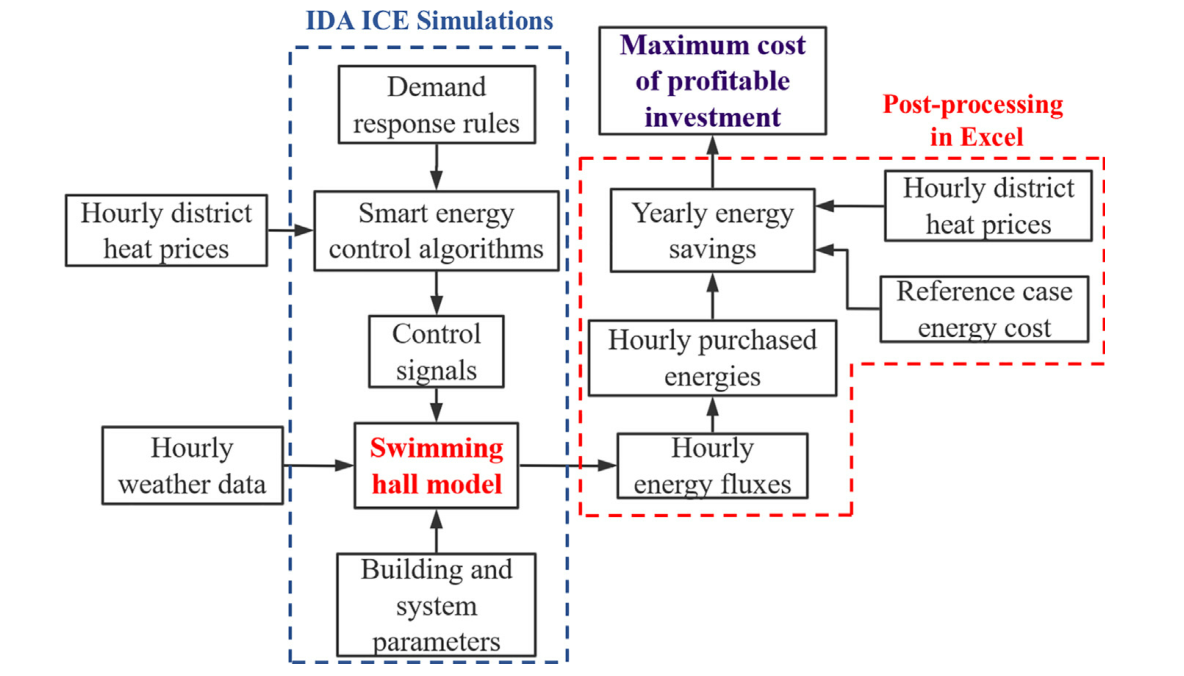
\includegraphics[scale=0.4]{figure_translate/1.png}
			\caption{论文逻辑结构图} \label{fig1}
		\end{figure*}
		\subsection{IDA ICE建筑能源分布仿真工具}
		IDA ICE是一个通用建筑模拟软件,该软件允许广泛的系统设计和配置,本文使用该软件建立游泳池模型。IDA ICE是一个适用于暖通空调系统、室外气候和内部热增益等建模的动态多区域模拟程序,可以同时实现质量流动和传热的动态模拟。已有多项研究成功验证了IDA ICE的可行性和可靠性,如文献\cite{article32,article33,article34}。
		\par
		IDA-ICE的泳池扩展程序,允许对某个区域内的水面进行建模,该扩展在本研究中使用。水池模型同时考虑了水面和区域之间的质量和热量传递。本文在扩展程序中模拟了在考虑了池水的连续补充的情况下,泳池达到和维持所选温度时池水的加热需求。
		\par
		\subsection{天气数据}
		测试参考年(TRY),根据历史天气数据再现赫尔辛基的典型年份,描述为芬兰南部当前的气候条件,并引入游泳池模拟模型\cite{article30}的IDA ICE。TRY包括打不限于温度,相对湿度、风速和风向以及赫尔辛基典型年份的直接正常和扩散水平表面上的太阳辐射根据\cref{fig2}所示,TRY温度范围为-20\textcelsius~30\textcelsius,湿度的范围为30\%~100\%。
		\par
		\subsection{动态能源价格}
		本文主要通过动态区域供热价格进行需求响应控制,尽管芬兰的区域供热价格本就随季节性或月度变化。本研究使用的动态区域供热价格代表芬兰某地区供热厂家的价格,包含能源、税收和动态的传输费。每小时的价格是根据一个由热电联产(CHP)电厂和热力锅炉组成的区域供热系统确定的,详见\cite{article19}。该价格是根据现有的每小时燃料价格数据计算出来的,并没有打算预测未来的地区热能价格。\cref{tab1}显示了动态区域供热价格的特性,而\cref{fig3}绘制了文章中使用的动态价格与芬兰地区供热厂家的随季节变化的区域供热价格的比较。
		\par 
		\begin{table}[H]
			\centering
			\caption{动态区域热价特性}
			\centering
			\begin{tabular}{*{4}{p{4em}}}
				\toprule    
				平均价格 & 标准差 & 标准差价格之比 & 超过平均价格比例\\
				\midrule
				50.63 & 23.24 & 46 & 20\% \\
				\bottomrule  
			\end{tabular}
			\label{tab1}
		\end{table}
		\par
		\begin{figure*}[htbp]
			\centering
			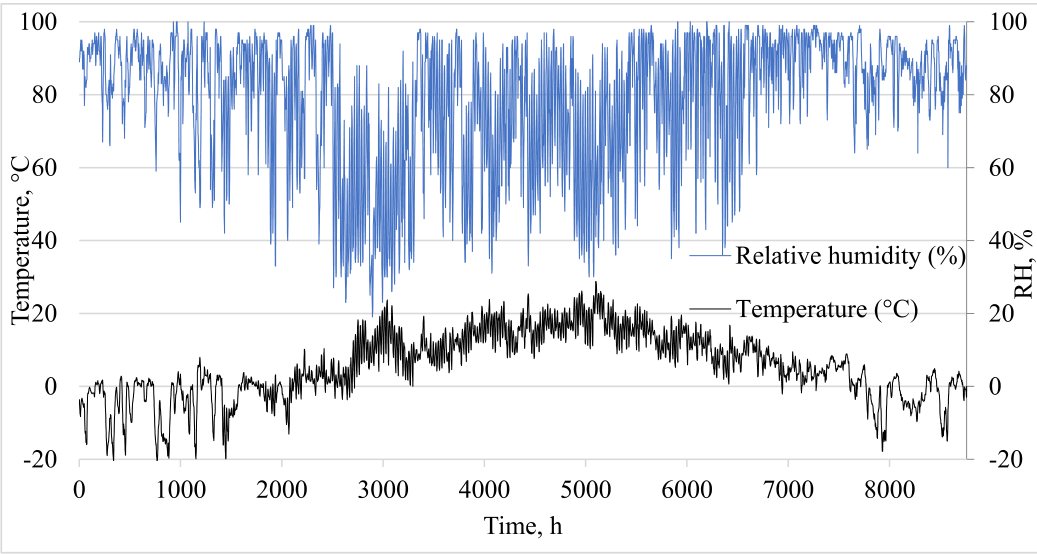
\includegraphics[scale=0.4]{figure_translate/2.png}
			\caption{TRY的温度和相对湿度(FMI, 2012)}
			\label{fig2}
		\end{figure*}
		\begin{figure*}[htbp]
			\centering
			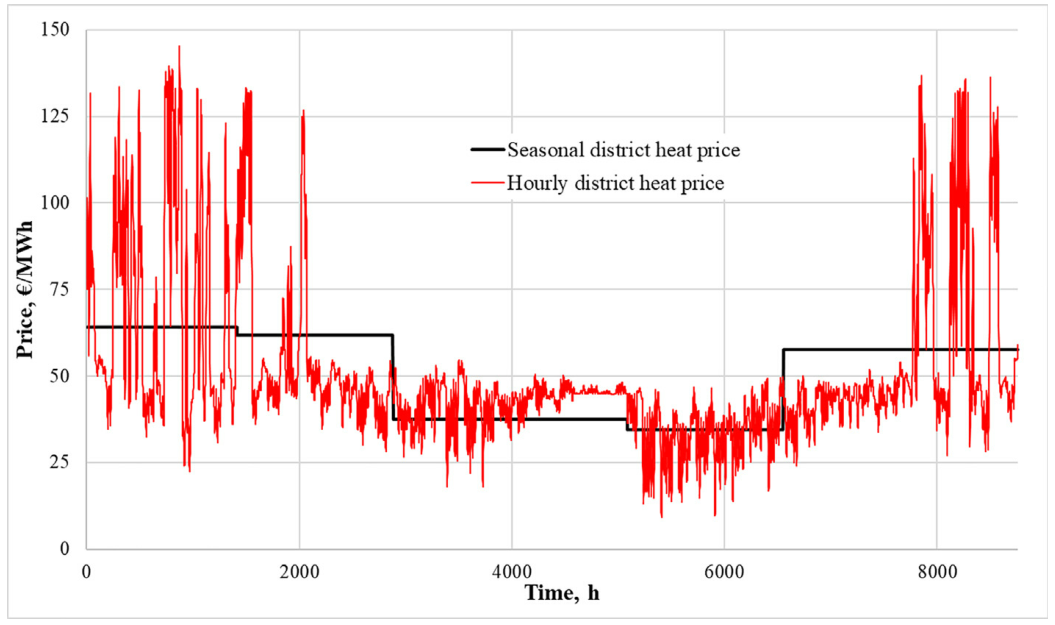
\includegraphics[scale=0.4]{figure_translate/3.png}
			\caption{研究中使用的每小时区域供热价格和芬兰区域供热供应商的季节性区域供热价格}
			\label{fig3}
		\end{figure*}
		\subsection{最大可盈利投资}
		最大可盈利投资的计算受到许多因素的影响,而本研究考虑了四个影响因素,即能源成本节约量、能源价格通胀、名义利率和还贷期限。\cref{tab2}给出了盈利投资最大成本的计算方法以及各变量的解释。还款期的定义是所实现系统假定的最小生命周期。本文采用能源价格年实际利率假设值为1\%,能源价格上涨2\%,采用7年、10年和15年三个还款期计算能源成本节约。
		\par
		\begin{table}[H]
			\centering
			\caption{盈利投资最大成本的计算方法}
			\begin{tabular}{ccp{10em}}
				\toprule    
				标号 & 等式 & 结果\\
				\midrule
				Eq.1 & $r_{e}=\frac{i-f_{e}}{1+f_{e}}$ & 能源价格的实际利率 \\
				Eq.2 & $a_{n}''=\frac{1-(1+r_{e})^{-n}}{r_{e}}$ & 总折扣收益率 \\
				Eq.3 & $S_{inv}=a_{n}''S_{E,a}$ & 盈利投资的最大成本(总能源成本节约)\\
				\bottomrule  
			\end{tabular}
			\label{tab2}
%			\tabnote{{\textbf{备注:}$r_{e}$ =能源价格年实际利率[\%];i=年名义利率[\%];$a_{n}''$=总折现率[a];n=还款期[a];$S_{inv}$=最大盈利投资成本[€];$S_{E,a}$=年度能源成本节约[€/a]。}
		\end{table}
		\section{游泳馆模型描述}
		\subsection{建筑特征}
		本文研究的游泳馆是芬兰赫尔辛基的是一个体育中心。所研究的游泳馆的几何形状和结构是根据赫尔辛基城市\cite{article36}的在线数据库和泳队教练得到的。本文利用Autodesk公司的AutoCAD MagiROOM软件,基于几何数据建立游泳馆模型。除所研究的游泳馆能耗数据外,还收集到大量综合综合数据应用于模型的建立。\cref{tab3}为所研究游泳馆模型外形参数,\cref{fig4}绘制所研究游泳馆模型的外形特征。
		\par
		在游泳馆模型中不同的U值是根据芬兰建筑规范\cite{article37}设定的(\cref{tab4})。由于窗户面积占总体结构的比例相对较大,围护结构的热损失受到窗户U值的显著影响。\cref{tab4}还显示了模拟中使用的参数,如热桥电导、50Pa压强下的漏风率($q_{50}$)和平均渗透率。
		\par
		\begin{table}[H]
			\centering
			\caption{游泳馆几何模型的主要特征值}
			\begin{tabular}{p{5em}ccp{3em}p{3em}}
				\toprule    
				\textbackslash & 面积 & 体积 & 窗户与整体面积之比 & 每平米对应面积\\
				\midrule
				Net floor & 7982 & \multirow{3}*{53463} & \multirow{3}{*}{8.9\%} & \multirow{3}{*}{0.26} \\
				Ground & 4047 & ~ & ~ & ~ \\
				Envelop & 13705 & ~ & ~ & ~ \\
				\bottomrule  
			\end{tabular}
			\label{tab3}
		\end{table}
		\begin{figure*}[htbp]
			\centering
			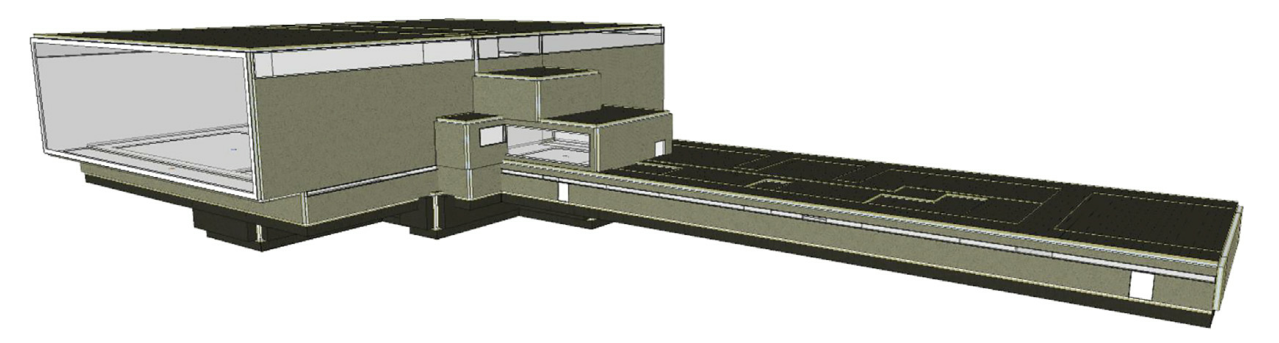
\includegraphics[scale=0.4]{figure_translate/4.png}
			\caption{游泳池的几何模型}
			\label{fig4}
		\end{figure*}
		\subsection{技术系统}
		\subsubsection{泳池信息}
		研究游泳馆共有主泳池、儿童泳池和幼儿泳池三个泳池,泳池表面积、平均深度、泳池水温等参数汇总如\cref{tab5}所示。根据ASHRAE(2003)\cite{article39},模型中大池、儿童池和幼儿池的蒸发系数分别为1、1.5和1。泳池模型的设计加热功率对每个泳池而言为200 $W/m_{2}$,设计供水温度为+37\textcelsius。此外,泳池的水温是根据最新测量的游泳池的平均温度设定的。
		\par
		\begin{table*}[htbp]
			\centering
			\caption{游泳馆几何模型的主要特征值}
			\begin{tabular}{llcccc}
				\toprule    
				泳池种类 & 使用方式 & 规模 & 泳池表面积 & 平均深度 & 水温\\
				\midrule
				主泳池   & 游泳健身 & 大泳池 & 400 & 2.8  & 26.5\\
				儿童泳池 & 游泳联系 & 大泳池 & 112 & 1.4  & 26.5\\
				幼儿泳池 & 儿童游乐 & 小泳池 & 63  & 0.75 & 28  \\
				\bottomrule  
			\end{tabular}
			\label{tab5}
		\end{table*}
		\subsubsection{空调机组}
		大泳池和儿童泳池共用一个AHU,而儿童泳池使用单独的AHU。\cref{fig5}显示了在IDA ICE中模拟的模拟游泳馆的两个AHU的示意图。两个泳池空间的供给气流速率由各自的VAV AHU和相对湿度(RH)调节。游泳池空间的AHU回收室内空气以使其相对湿度处于50\%至57\%之间,而相应的每净地板面积的送风气流在2 $dm_{3}/s/m_{2}$到4$dm_{3}/s/m_{2}$之间。主泳池室内空气采暖设定值为+28\textcelsius,供风采暖温度在+25\textcelsius~ +37\textcelsius 之间,儿童水池室内空气采暖设定值为+30\textcelsius。根据Hemmilä和Laitinen\cite{article22},热回收的温度效率为60\%。
		\par
		\begin{table}[H]
			\centering
			\caption{游泳馆模型的包络参数}
			\begin{tabular}{ccc}
				\toprule    
				参数 & 值 & 地点\textbackslash 备注 \\
				\midrule
				结构的U值 & & \\
				-窗户 & 1.0 & 全空间\\
				-基板 & 0.24 & 全空间\\
				-天花板 & 0.2 & 全空间\\
				-外墙 & 0.23 & 全空间\\
				\midrule
				\multirow{2}*{-内墙} & 0.47 & 泳池区域\\
				~ & 0.8 & 其他区域\\
				\midrule
				\multirow{4}{*}{热桥电导} & 0.08 & 天花板\textbackslash 外墙\\
				~ & 0.24 & 基板\textbackslash 外墙\\
				~ & 0.06 & 外墙\\
				~ & 0.03 & 外部门窗\\
				\midrule
				漏风率 & 3.3 & \\
				平均渗入率 & 0.04 & 每小时换气\\
				\bottomrule  
			\end{tabular}
			\label{tab4}
		\end{table}
		淋浴房和其他空间都有自己的变风量控制的AHU,其送风率根据空间的二氧化碳水平调整。暖室空调系统送风温度为+16\textcelsius,淋浴房空调系统送风温度为+13\textcelsius ~ +30\textcelsius,受室内空气温度影响。\cref{tab6}显示了通风系统的设定加热温度和性能。
		\par
		\begin{table*}[htbp]
			\centering
			\caption{游泳池模型中加热系统的设计温度和加热功率}
			\begin{tabular}{lccccc}
				\toprule    
				AHU区域 & 净面积 & 室内设定加热温度 & 最小室外气流 & 最大室外气流 & 热回收效率\\
				\midrule
				主泳池   & 1144 & 28 & 2.0 & 4.0 & 60\\
				幼儿泳池 & 231 & 30 & 2.0 & 4.0 & 60\\
				洗澡区域 & 411 & 24 & 3.3 & 6.7 & 60  \\
				其他区域 & 6196 & 18 & 0.5 & 2.6 & 60 \\
				\bottomrule  
			\end{tabular}
			\label{tab6}
		\end{table*}
		\begin{figure*}[htbp]
			\centering
			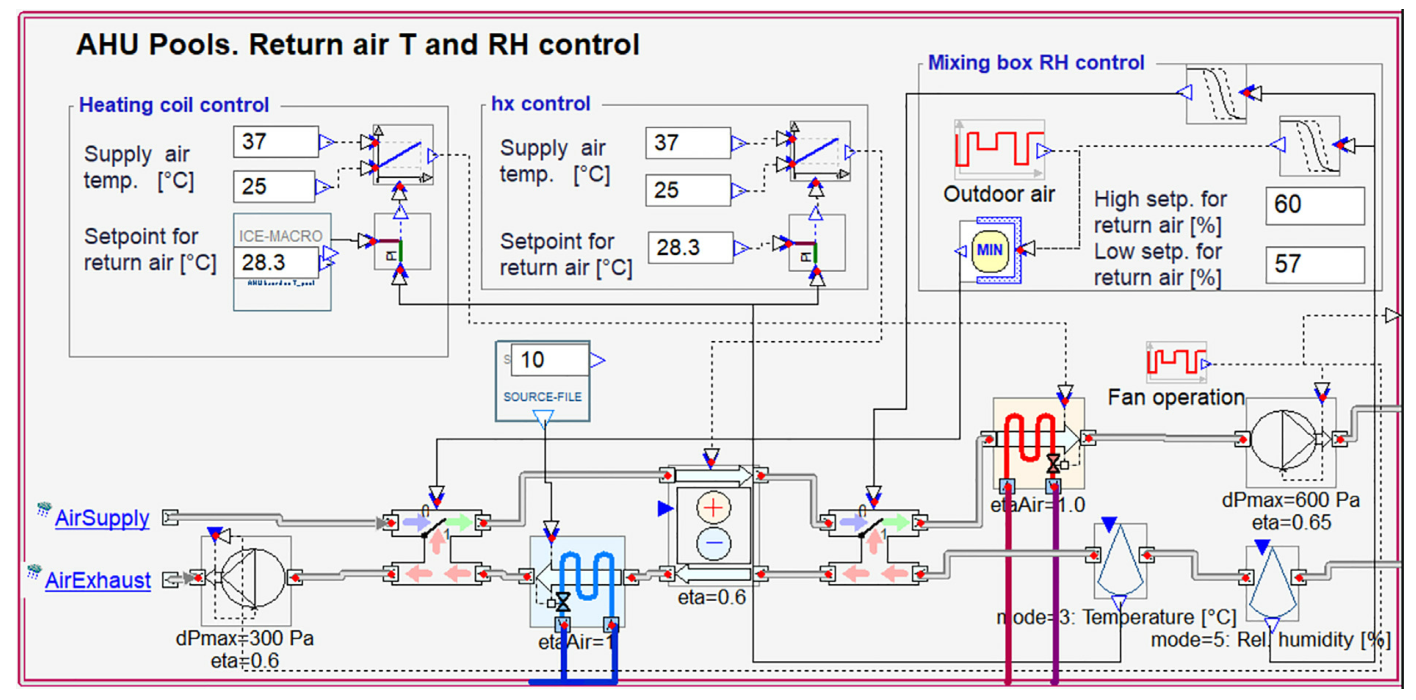
\includegraphics[scale=0.4]{figure_translate/5.png}
			\caption{游泳池的几何模型}
			\label{fig5}
		\end{figure*}
		\subsubsection{DHW的使用和加热系统}
		DHW设定加热温度为+55\textcelsius,用于能量计算的冷水温度设为+8\textcelsius。根据\cite{article22}和\cite{article40},平均自来水温度和平均DHW使用量是+39\textcelsius 和51$m_{3}/天$。\cref{tab7}为所研究的游泳馆模型的设计温度和加热功率。除淋浴间外,所有空间均采用水散热器供暖,而泳池和淋浴间均采用地暖。
		\par
		\begin{table}[H]
			\centering
			\caption{游泳池模型中加热系统的设计温度和加热功率}
			\begin{tabular}{ccc}
				\toprule    
				加热系统 & 设计温度 & 设计温度功率\\
				\midrule
				\multirow{3}{*}{池水辐射供暖} & \multirow{3}{*}{50\textbackslash 30}  & 主泳池:40\\
				~ & ~ & 小泳池:6\\
				~ & ~ & 淋浴:24\\
				\multirow{2}{*}{地暖} & \multirow{2}{*}{34\textbackslash 30} & 主泳池:23\\
				~ & ~ & 小泳池:5\\
				泳池加热 & 40\textbackslash 27 & 400kW\\
				\bottomrule  
			\end{tabular}
			\label{tab7}
		\end{table}
		\subsection{使用时间表}
		\begin{table}[H]
			\centering
			\caption{每周泳池使用率和DHW使用情况}
			\begin{tabular}{cp{6em}c}
				\toprule    
				时段 & 开放时间 & 使用率\\
				\midrule
				\multirow{2}{*}{工作日} & 7点到16点,21点半到22点半 & 25\% 使用效率\\
				~ & 16点到21点 & 75\% 使用效率\\
				\midrule
				\multirow{4}{*}{周末节假日} & 7点到9点,21点半到22点半 & 25\% 使用效率\\
				~ & 9点到10点 & 50\% 使用效率\\
				~ & 20点半到21点半 & 75\% 使用效率\\
				~ & 10点到20点半 & 100\% 使用效率\\
				\bottomrule  
			\end{tabular}
			\label{tab8}
		\end{table}
		游泳馆每年7月14日至5月31日开放,每天开放时间为上午7点至晚上10点半。在工作日,游泳馆模型的照明安排分为三个部分,在上午7点至下午16点之间半功率运行。在其他时间段全功率运行并在关闭时间切断电源。\cref{tab8}显示了每周占用率和DHW每周使用情况。游泳馆的观众看台最多可容纳300人,但这种集会只会在每2个月18到21日中的周日举行一次。在18日至21日的其他周日,观众看台有10\%的观众,而观众看台在休息时间关闭。桑拿房的供暖系统是根据游泳馆的开放时间提供的。
		\par
		\section{能源系统的智能控制}
		\subsection{包含系统}
		本文中游泳馆能源系统的智能控制是指利用动态区域供热价格进行需求响应控制。游泳池的热容可以通过需求响应来利用。本研究使用的控制策略是调节全局温度,设定温度是根据全局控制信号进行调整。游泳馆内的热舒适应该通过适当的设定温度来保证到一个可接受的水平。
		\par
		\begin{table}[H]
			\centering
			\caption{大水池和儿童水池蓄热和排热的温度变化}
			\begin{tabular}{lccp{5em}}
				\toprule    
				加热能源 & 主泳池 & 儿童泳池 & 备注\\
				\midrule
				最大贮存热值 & 4570 & 640 & 泳池温度从26.5\textcelsius 升至 30\textcelsius \\
				最小储存热值 & 2653 & 91  & 泳池温度从26.5\textcelsius 升至 26\textcelsius  \\
				\bottomrule  
			\end{tabular}
			\label{tab9}
		\end{table}
		在研究的游泳馆中,主要水池(大水池和儿童池)的水温通过负荷转移策略和区域热需求响应控制。主池的温度设定点是相同的,最小值为26\textcelsius,正常值为26.5\textcelsius,最大值为30\textcelsius。\cref{tab9}显示了在游泳池水完全混合的情况下,大型游泳池和儿童游泳池池水温度变化造成的蓄排热量情况。当泳池水温从26.5\textcelsius 升高到30\textcelsius 时,大型泳池和儿童泳池的最大蓄热分别约为4570和640 KWh。当池水温度从26.5\textcelsius 降至26 \textcelsius 时,大水池和儿童水池释放的最大热量分别约为640和91KWh。室内空气与泳池水温差大会造成室内结露,因此泳池水的温度设定值总是比室内空气低2\textcelsius。温度传感器持续监控可循环池中回水温度的变化,根据水温设定空气加热温度。
		\par
		\subsection{控制算法}
		本文采用以动态区域供热价格为参数的基于规则的控制算法对游泳馆能源系统进行控制。控制算法的目的是为能源系统提供控制信号,以达到降低能耗或节约能源成本的目的,而设置控制信号是为了实现对影响能源系统加热功率的设定温度值的调整。
		\par
		本文采用区域动态供热价格对需求响应系统进行控制。系统温度设定值在区域热价高的情况下降低,在区域热价低的情况下升高。因此,确定便宜和昂贵的区域供热价格的时间占总时间的百分比是重要的,影响着如何设置系统温度。\cref{fig6}为全年区域供热每小时价格的持续时间长度曲线,虚线分别代表8\%、20\%和30\%的区域供热价格剔除比例。剔除比例的选择是灵活的,其目的是根据持续时间曲线将地区供热价格划分为三个价格水平。从\cref{fig6}可以看出,近20\%的区域供热价格明显高于其余的价格;因此,选择20\%作为游泳池热水的高限价(HPL)百分比。同样的百分比(20\%)也被选为低价格限制(LPL)。
		\par
		\begin{figure*}[htbp]
			\centering
			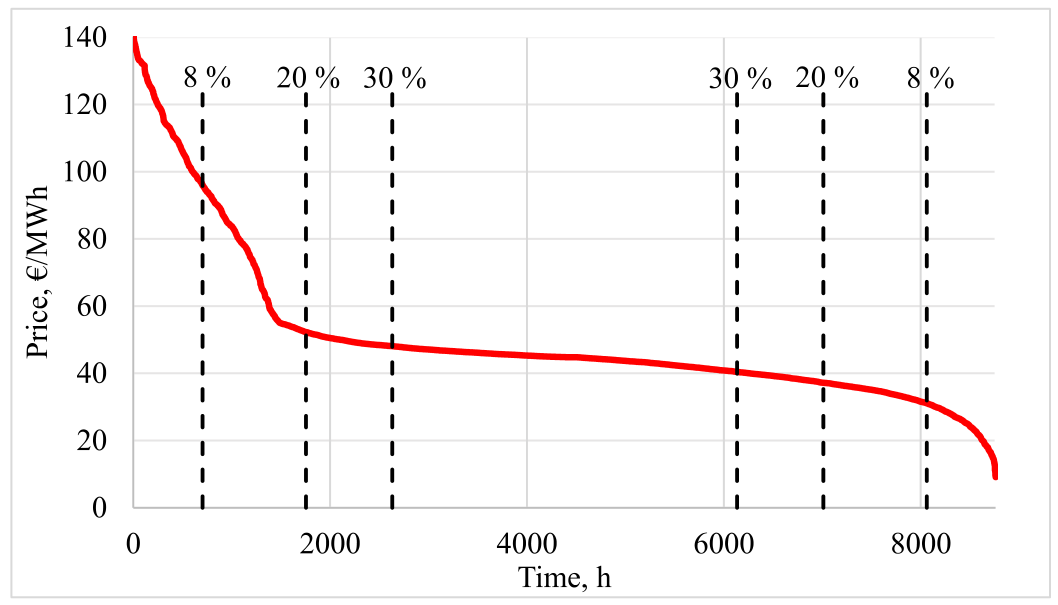
\includegraphics[scale=0.4]{figure_translate/6.png}
			\caption{游泳池的几何模型}
			\label{fig6}
		\end{figure*}
		本文所开发的算法定义了当前能源价格(CEP)的状态,即当前区域供热价格。当前能源价格的状态分为昂贵、正常和便宜。\cref{fig7}所示为动态能源价格决策算法、输入数据和输出数据。算法有三个输入,三个已经确定的比例,8\%,20\%和30\%为使总价中含有最少比例的昂贵的和便宜的价格,过去两周和未来12小时的区域供热价格由假设已知的价格提前12h得出。算法输出为-1,0和1的控制信号,分别表示当前能源价格的昂贵、正常和廉价状态。该算法的目的是对昂贵和便宜的地区供热价格的最小百分比进行分类。算法设置了价格上限(HPL)和价格下限(LPL),并将当前能源价格的价格等级与上下限进行了比较。
		\par
		\begin{figure*}[htbp]
			\centering
			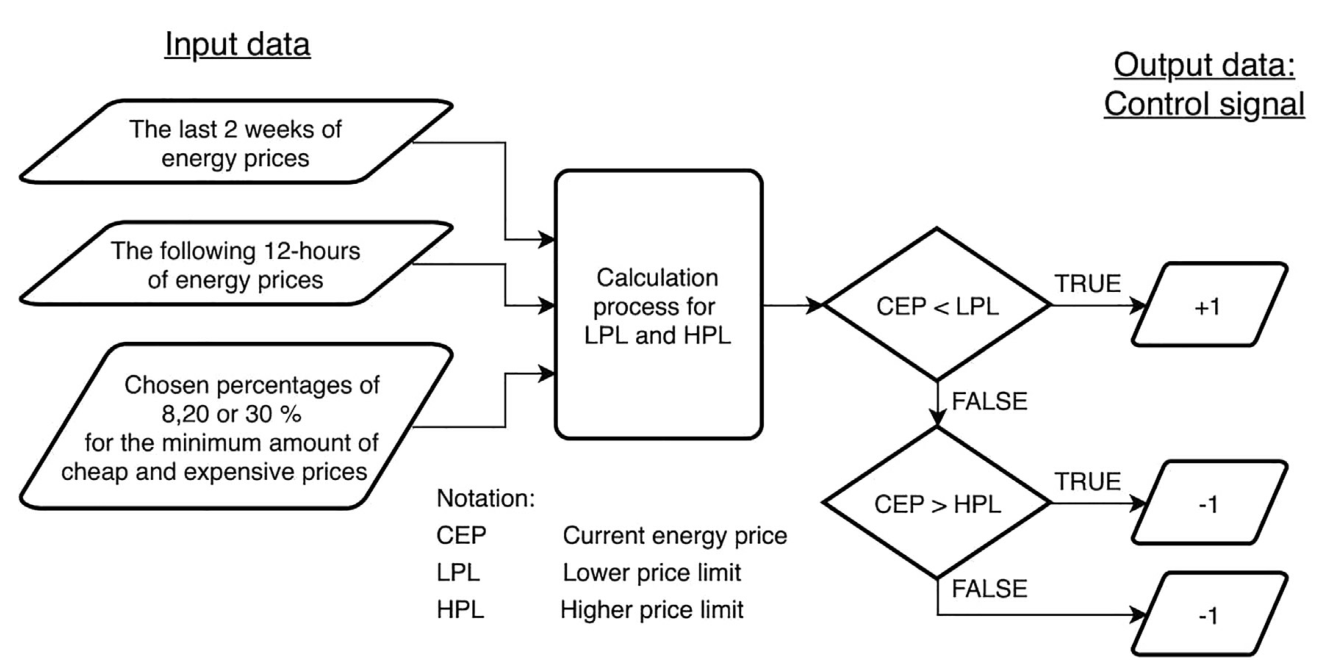
\includegraphics[scale=0.4]{figure_translate/7.png}
			\caption{游泳池的几何模型}
			\label{fig7}
		\end{figure*}
		\cref{fig8}为过去两周能源价格动态示例,以及接下来12小时的预测价格数据、当前能源价格、当前价格上限和当前价格下限。\cref{fig8}所示例子中的瞬时控制信号为+1,说明当前能源价格被归为便宜。\cref{tab10}显示了基于控制信号的温度设定值和全年设定值的活跃百分比。
		\par
		\begin{table}[H]
			\centering
			\caption{设定温度和设定点活动百分比}
			\begin{tabular}{p{10em}ccc}
				\hline    
				游泳馆区域供热需求响应 & 保守 & 正常 & 负载\\
				\hline  
				设定温度 & 26\textcelsius & 26.5\textcelsius & 30\textcelsius\\
				占比 & 32\% & 38\% & 30\% \\
				\hline   
			\end{tabular}
			\label{tab10}
		\end{table}
		\begin{figure*}[htbp]
			\centering
			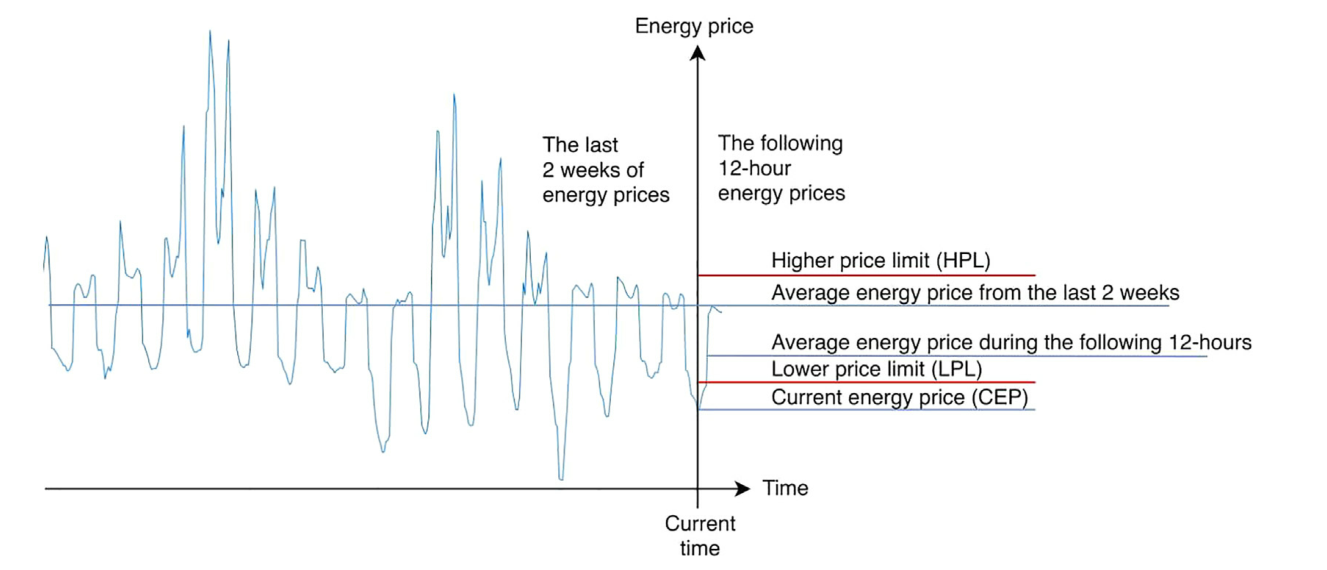
\includegraphics[scale=0.4]{figure_translate/8.png}
			\caption{游泳池的几何模型}
			\label{fig8}
		\end{figure*}
		\cref{fig9}为基于12月(样例时段)游泳馆区域热需求响应下控制的泳池水温设定点。由于区域供热动态价格的不可预测性,一个均匀的温度设定点将会有很大的周期跨度,其差异从几个小时到几天不等。由于研究游泳馆的热容较大,将泳池温度加热到较高的温度设定值需要较长时间。因此,短时间的高温对实际池水温度影响不大,而池水温度对需求响应动作的反应非常缓慢。
		\par
		\begin{figure*}[htbp]
			\centering
			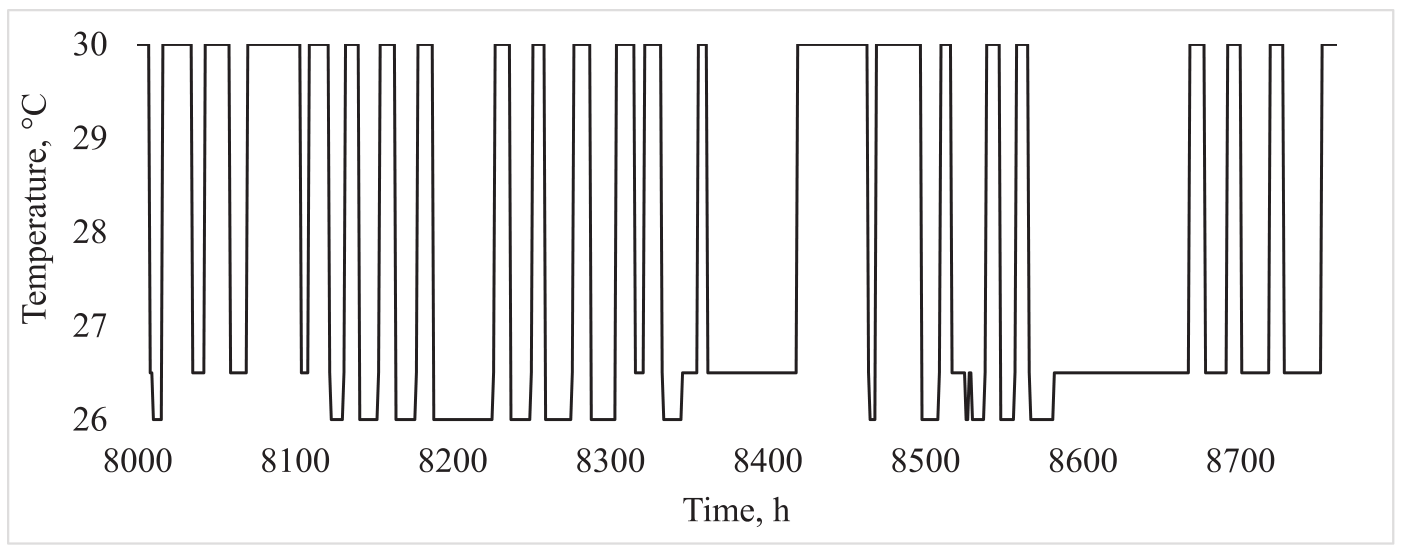
\includegraphics[scale=0.4]{figure_translate/9.png}
			\caption{游泳池的几何模型}
			\label{fig9}
		\end{figure*}
		\section{结果}
		\subsection{算例描述}
		除6月1日至7月13日暑假外,文中游泳馆全年大部分时间开放,所以游泳馆模拟期为每年322天。本文有两种情况,即参考情况1和需求响应的最优情况2。参考案例1对室内设置恒定温度(见\cref{tab6})并保持池水维持某一恒定水平不变(见\cref{tab9})。与参考案例1相比,第2种情况应用基于需求响应控制游泳池和室内空气温度。在情况2中,泳池水温设定点为26\textcelsius~30\textcelsius,而室内空气的设定温度都控制的比泳池水温高2\textcelsius,以防止凝露。
		\par
		\subsection{需求响应对池水和区域热动力的影响}
		大水池的表面积是儿童水池的4倍,造成了更高的热需求和热损失。同时,大池的平均深度是儿童池的两倍。因此,大水池单位体积的热量散失大约是儿童水池的两倍,导致水温变化较慢。大池对水温变化反应缓慢,增加了需求响应的潜力。因此,本节以大水池为例对水池水温和水池总加热功率进行了分析。
		\par
		\cref{fig10}比较了工况1和工况2全年(包括夏季休假)大泳池每小时水温的变化情况。在工况1中,所有池水温度在正常设定值(26.5\textcelsius)附近徘徊,其偏差不超过$\pm0.5$\textcelsius。然而,工况2中的池水温度在保存温度(26\textcelsius)和负载温度(30\textcelsius)之间。主泳池的平均温度从正常的26.5\textcelsius 上升到27.3\textcelsius。在工况2中,上半年的平均温度(27.5\textcelsius)高于下半年的平均温度(27.1\textcelsius)。这种不均匀的全年平均气温主要是由区域供暖趋势主导的,其价格在上半年下降,在其余半年上升。更先进的算法可以帮助避免长时间的高水温和补偿平均温度不均匀的影响。
		\par
		\begin{figure*}[htbp]
			\centering
			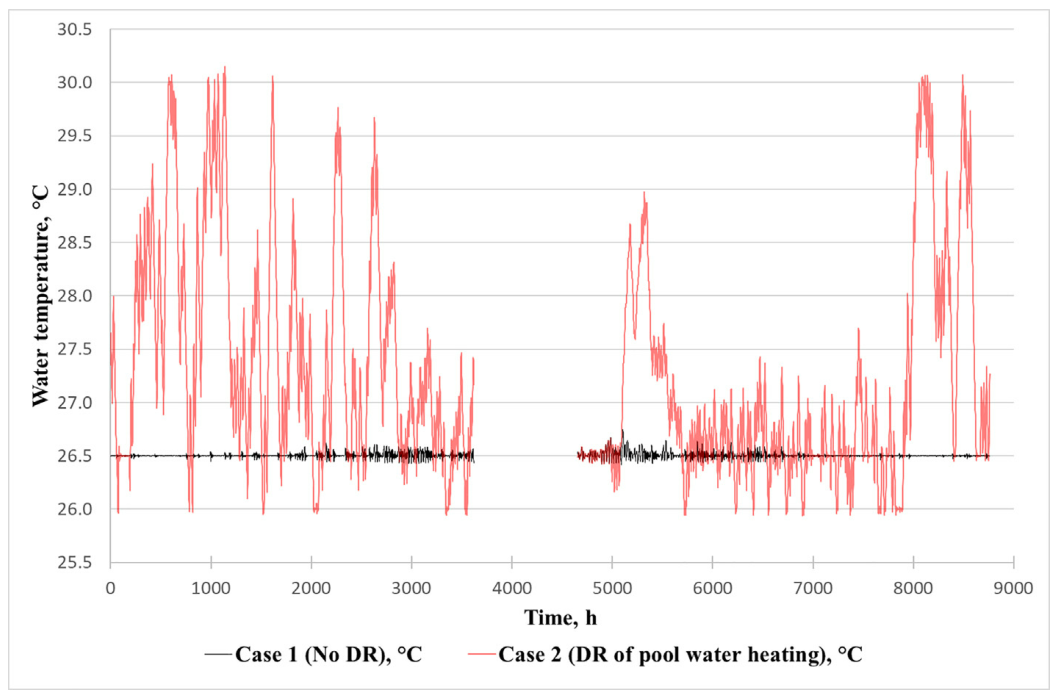
\includegraphics[scale=0.4]{figure_translate/10.png}
			\caption{游泳池的几何模型}
			\label{fig10}
		\end{figure*}
		\cref{fig11}为工况1与工况2大泳池水温持续时间曲线对比图。由\cref{tab9}可知,保存、正常和负载设定点温度的激活百分比分别为32\%、38\%和30\%。大约80\%的实际水温在正常值和负载值之间,而20\%的实际水温在保守值和正常值之间。与工况1相比,工况2在整个模拟期间大池中储存的热能约为8120MWh,而工况2释放的热能大约是400MWh。游泳馆池的大水贮水量保证了可充放热能的储存。
		\par
		\begin{figure*}[htbp]
			\centering
			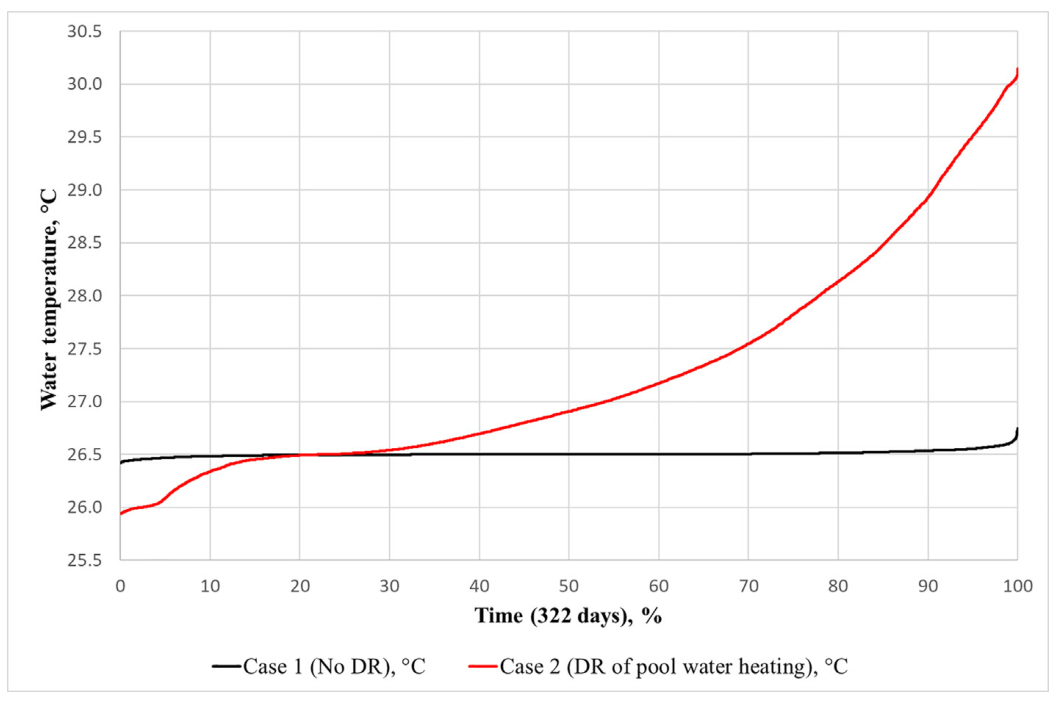
\includegraphics[scale=0.4]{figure_translate/11.png}
			\caption{游泳池的几何模型}
			\label{fig11}
		\end{figure*}
		\cref{fig12}比较了工况1和工况2的区域供热下每小时池水加热功率。在冬季,情形2池水区域每小时加热功率与工况1相比有显著差异。需要注意的是,因为已开发的需求响应根据区域供热厂家定义的价格信号来控制存储和释放热量,所以大厅区域供热电力需求的变化程度增加。这样,游泳馆在区域热网络中像一个能量存储体使得网络的灵活性提高。
		\par
		\begin{figure*}[htbp]
			\centering
			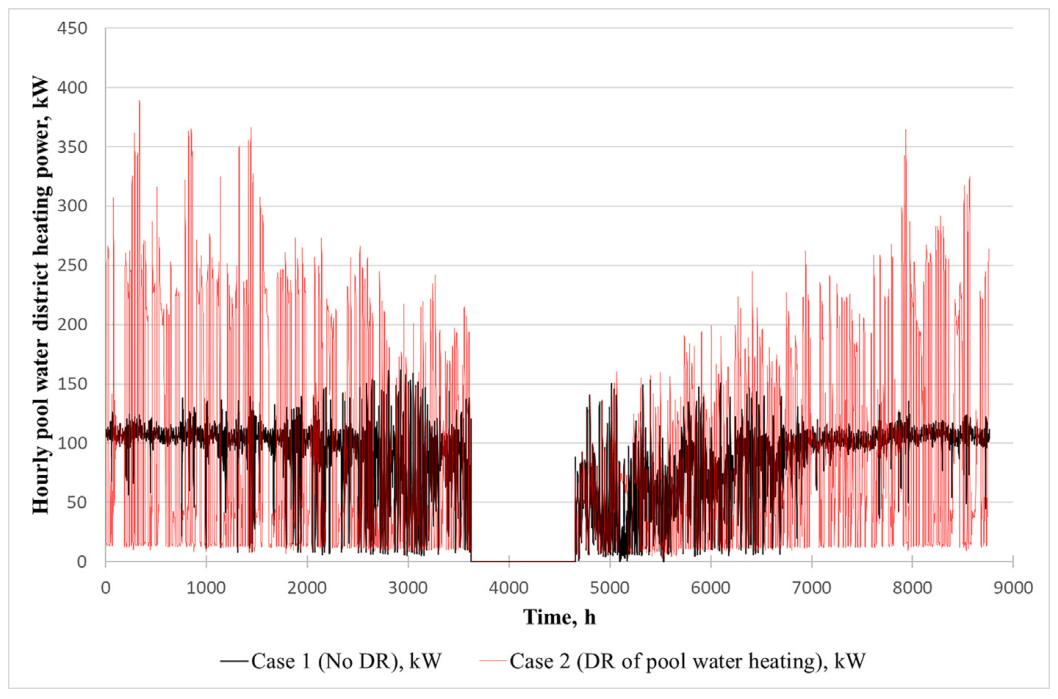
\includegraphics[scale=0.4]{figure_translate/12.png}
			\caption{游泳池的几何模型}
			\label{fig12}
		\end{figure*}
		\cref{fig13}对比了工况1和工况2的总池水区域加热功率持续时间曲线。在工况1和工况2中,池水的最大区域加热功率分别约为160kW和390kW。在全年64\%的时段内,工况1的池水集中供热功率大于工况2,其差异均在80kw以下。但在全年其余36\%的时间里,情形2的池水区域加热功率大于情形1,最大差异在230kW左右。虽然情形2的池水区域加热功率在64\%全年期间小于情形1,但情形2的水温在80\%全年期间可以保持高于情形1的温度(如\cref{fig11}所示)。
		\par
		\begin{figure*}[htbp]
			\centering
			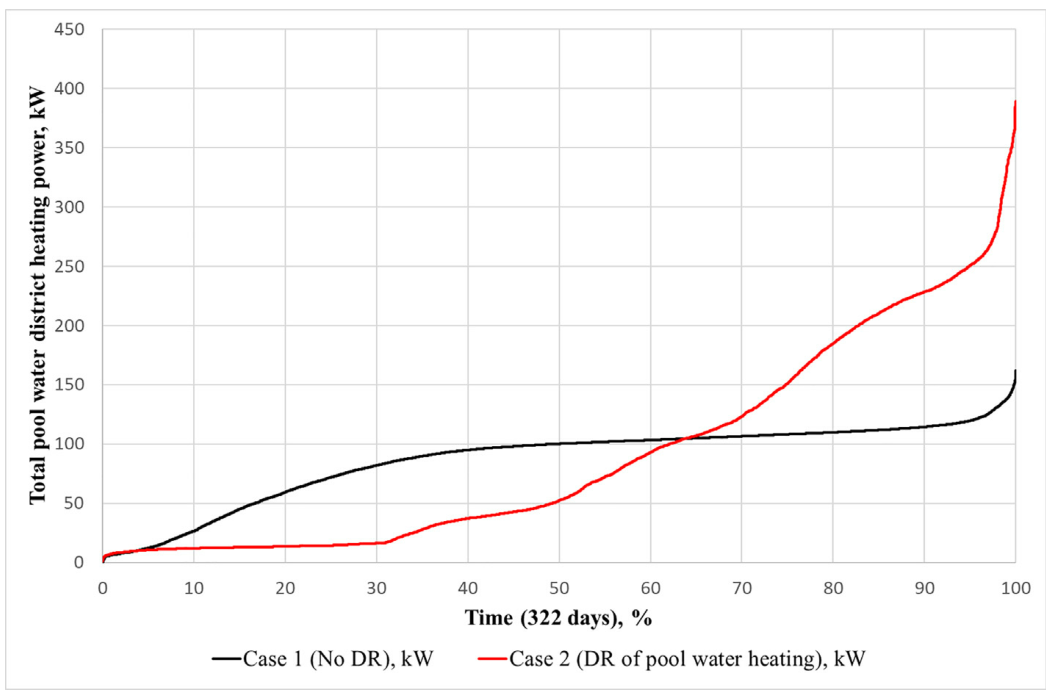
\includegraphics[scale=0.4]{figure_translate/13.png}
			\caption{游泳池的几何模型}
			\label{fig13}
		\end{figure*}
		\subsection{区域年耗热量的分解}
		\cref{tab11}分别为工况1和工况2各能源系统每年区域热能消耗情况。采购的集中供热用于空间采暖、送风采暖、DHW加热和池水加热,而消耗热量最大的是DHW加热,其次是泳池水加热。
		由\cref{tab11}可知,工况1年采购区域热总量为2717 MWh/a,工况2年采购区域热总量为2764 MWh/a。在工况2下,保持室内空气设定温度比池水温高2\textcelsius,使采购的总区域热量增加1.7\%,加热池水消耗热量增加5.5\%。
		\par
		\begin{table}[H]
			\centering
			\caption{年度能源和能源成本比较}
			\begin{tabular}{ccc}
				\toprule
				\multirow{2}{*}{能源系统} & \multicolumn{2}{c}{区域供热} \\
				\cmidrule{2-3}
				~ & 情况1 & 情况2 \\
				\midrule
				空气供热 & 614 & 629 \\
				区域供热 & 458 & 453 \\
				DHW供热 & 976 & 976\\
				泳池供热 & 669 & 706\\
				总计 & 2717 & 2764\\
				\bottomrule
			\end{tabular}
			\label{tab11}
		\end{table}
		\subsection{能源成本和盈利投资的最大成本}
		\cref{tab12}比较了参考案例(工况1)和需求响应下(工况2)的年能源成本。工况2中每年购买的区域供热量与工况1非常接近,在对照情况下,购买热量从2717MWh/a增加到2764MWh/a,增加了47MWh/a,而它们之间的相对变化只有+1.7\%。需求响应的目的不是改变系统中的能源用量,而是管理需求侧的能源使用。每年购买地区供热的费用包括各项费用和增值税。与对照案例中购买区域供热的155000欧元年度成本相比,工况2为153000欧元,每年减少2000欧元,节能率约为1.1\%。
		\par
		\begin{table}[H]
			\centering
			\caption{年度能源和能源成本比较}
			\begin{tabular}{lcc}
				\toprule
				\multirow{2}{*}{案例} & 参考 & 需求响应 \\
				~ & 情况1 & 情况2 \\
				\midrule
				年采购区热 & 2717 & 2764 \\
				年能量的绝对变化 & - & +47 \\
				年能量的相对变化 & - & +1.7\\
				购买区域供热的年度成本 & 155000 & 15300\\
				年能源成本的绝对变化 & - & -2000\\
				每年能源成本的相对变化 & - & -1.1\\
				\bottomrule
			\end{tabular}
			\label{tab12}
		\end{table}
		分别设定三个还款期,7年、10年、15年,在该条件下计算盈利投资的最大成本,计算方法见第3.0节。游泳馆的需求响应每年节省能源成本2000欧元。需求响应下,游泳池的最大可盈利投资成本在10000欧元(7-10年还款期)和20000欧元(15年还款期)之间。
		\par
		\section{分类讨论}
		游泳馆属于建筑行业,需要良好的室内空气条件,能耗较大\cite{article14}。截至2018年,芬兰共有280个游泳馆,而过去10年平均每年增加2个游泳馆。游泳馆的增长趋势还将继续下去。此外,许多旧的游泳馆需要改造以满足现代法规,减小能源损耗。芬兰新建和改造游泳馆的巨大需求为游泳馆实施智能和可持续能源系统带来了潜力。
		\par
		近年来,需求响应已成为电力市场上一个很有前途的概念,并被广泛应用于建筑能源系统中,以达到节约能源成本和平衡供需双方的目的\cite{article41}。需求响应通过特定的算法调节温度设定值使游泳馆需求响应系统的投资成本较小。游泳馆能量系统具有较大的蓄热能力,因此推荐采用集中供热。采用需求响应控制的重型混凝土结构建筑为能源生产提供了灵活性与潜力。游泳馆有较高的灵活性和需求响应潜力,因为它们通常是用混凝土等重型建筑材料建造的,游泳池的水自带的超大热容也可以用于游泳馆的需求响应。因此,一个需求响应控制的游泳馆可以作为一个集中供热网络的能量存储点,并减少峰值时期发电厂的使用,从而减少二氧化碳排放。
		\par
		值得注意的是,研究中使用的动态热量价格是基于现有的每小时燃料价格数据计算来的,没有考虑到区域供热厂家的灵活性。如果一个区域供热厂家因为增加了灵活性而获得额外的利润且与客户共享利润,那么客户可节省的成本可能比研究中显示的要高。
		\par
		需求响应在游泳馆能量系统中的应用还没有进行过研究;因此,本研究具有很强的创新性,值得进一步深入研究。由于本文的算法没有进行优化,未来的研究可以比本研究实现更大的潜在能源成本节约。未来研究的重点可能是优化游泳馆或其他体育中心的需求响应方法和算法,例如滑冰馆和体育馆,从客户和能源厂家的角度考虑。游泳馆由于其巨大的热需求和容量,具有巨大的区域热需求响应潜力。未来应提出和研究更精确的游泳馆能源系统智能控制,挖掘需求响应控制在节能减排、降低成本方面的潜力。此外,游泳池用电与区域供热的需求响应耦合控制问题也应被注意,如热泵同时用于区域供热和供热时的需求响应问题。
		\par
		\section{结论}
		本文提出了一种需求响应理论将其应用于芬兰某游泳馆的能量系统中。研究过程分为两部分,使用IDA ICE工具进行动态仿真和使用Excel 2016对仿真结果进行后处理。游泳馆模拟模型的输入包括研究的游泳馆数据、假设模型参数、当地每小时天气数据和该地区每小时供热价格。本文的重点是将基于规则的需求响应算法应用于研究的游泳馆以实现区域热需求响应,其中降低峰值负荷和负荷转移是本文研究的两个需求响应概念。结论如下:
		\par
		\begin{enumerate}	
			\item 游泳馆池水储水量大,保证了可以储存和释放大量的热能以供不时之需,增加了集中供热网络的灵活性。
			\item 区域热需求响应的应用可以使全年池水平均温度由正常的26.5\textcelsius 提高到27.3\textcelsius。
			\item 需求响应控制的集中供热可以降低平均购买的集中供热价格和总能源成本。在对泳池水和室内气温进行区域热需求响应的游泳馆中,相应的区域供热成本节约达到1.1\%。
			\item 在7年和15年的还款期,需求响应控制的可盈利的投资成本节约在1万欧元到2万欧元之间。
		\end{enumerate}
		\section*{感谢}
		这项研究是HUKATON和FINEST Twins项目“建筑环境中高效余热回收和热存储的新商业和合作模式”的一部分。HUKATON项目由欧洲区域发展基金(ERDF)、赫尔辛基市和海伦有限公司资助,FINEST Twins项目由欧盟(Horizon 2020项目,批准号856602)和爱沙尼亚政府共同资助。本文也获得了国家自然科学基金(批准号51978481)的资助。
		\par
		\begin{thebibliography}{100}%此处数字为最多可添加的参考文献数量
			\bibitem{article1} European Commission 2017, Energy efficiency - Buildings. [Online]. Available: https://ec.europa.eu/energy/en/topics/energy-efficiency/buildings.
			\bibitem{article2} Z. Li, Y. Han, P. Xu, Methods for benchmarking building energy consumption against its past or intended performance: An overview, Appl. Energy 124 (2014) 325–334. 
			\bibitem{article3} L. Yang, H. Yan, J.C. Lam, Thermal comfort and building energy consumption implications – A review, Appl. Energy 115 (2014) 164–173.
			\bibitem{article4} X. Yuan, M. Shahrestani, D. Fernbank, J. Burton, L. Liu. Y. Yang, Performance characteristics of ground source heat pump and combined heat and power systems under electricity decarbonisation plans. In: The 8th International Conference of SuDBE2017, 4-7 Nov 2017, Chongqing, China. 
			\bibitem{article5} B. Parrish, P. Heptonstall, R. Gross, B.K. Sovacool, A systematic review of motivations, enablers and barriers for consumer engagement with residential demand response, Energy Policy 138 (2020) 111221. 
			\bibitem{article6} M. Hussain, Y. Gao, A review of demand response in an efficient smart grid environment, Electr. J. 31 (2018) 55–63. 
			\bibitem{article7} W. Li, L. Yang, Y. Ji, P. Xu, Estimating demand response potential under coupled thermal inertia of building and air-conditioning system, Energy Build. 182 (2019) 19–29. 
			\bibitem{article8} B. Cui, S. Wang, C. Yan, X. Xue, Evaluation of a fast power demand response strategy using active and passive building cold storages for smart grid applications, Energy Convers. Manage. 102 (2015) 227–238.
			\bibitem{article9} F.E.R. Commission, 2010, Assessment of Demand Response and Advanced Metering, United States Department of Energy, Washington DC, USA, 2011. 
			\bibitem{article10} M.H. Albadi, E.F. El-Saadany, A summary of demand response in electricity markets, Electr. Power Syst. Res. 78 (2008) 1989–1996. 
			\bibitem{article11} L. Shen, Z. Li, Y. Sun, Performance evaluation of conventional demand response at building-group-level under different electricity pricings, Energy Build. 128 (2016) 143–154. 
			\bibitem{article12} P. Cappers, C. Goldman, D. Kathan, Demand response in U.S. electricity markets: Empirical evidence, Energy 35 (4) (2010) 1526–1535. 
			\bibitem{article13} K. Martin, Demand response of heating and ventilation within educational office buildings. Master’s Thesis. Aalto University, Espoo, Finland, 2017. Available: http://urn.fi/URN:NBN:fi:aalto-201712187947. 
			\bibitem{article14} Finnish energy. 2018. Energiavuosi 2017 - Kaukolämpö (Energy year 2017 District heating). [Online]. [Cited 28.8.2018]. Available from: https://energia.fi/ ajankohtaista_ja_materiaalipankki /materiaalipankki/energiavuosi_2017__kaukolampo.html. 
			\bibitem{article15} S. Frederiksen, S. Werner, District heating and cooling, 1.th ed., Studentlitteratur AB, Lund, Sweden, 2013, p. 586. 
			\bibitem{article16} B. Vand, K. Martin, J. Jokisalo, R. Kosonen, A. Hast. Demand response potential of district heating and ventilation in an educational office building. Science and Technology for the Built Environment. 2019. (Available: https://doi.org/ 10.1080/23744731.2019.1693207). 
			\bibitem{article17} A. Mäki, Demand response of space heating using model predictive control in an office building. Master’s Thesis. Aalto University, Espoo, Finland, 2018. [Published] 
			\bibitem{article18} T. Sweetnam, C. Spataru, M. Barrett, E. Carter, Domestic demand-side response on district heating networks, Build. Res. Inf. 47 (2019) 330–343. 
			\bibitem{article19} S. Salo, A. Hast, J. Jokisalo, R. Kosonen, S. Syri, J. Hirvonen, K. Martin, The impact of optimal demand response control and thermal energy storage on a district heating system, Energies 12 (9) (2019).
			\bibitem{article20} P. Ala-Kotila, T. Vainio, J. Heinonen, Demand response in district heating market—results of the field tests in student apartment buildings, Smart Cities 3 (2020) 157–171. 
			\bibitem{article21} L. Lindroos, Waste heat utilization and smart energy system of combined ice and swimming halls. Master’s Thesis. Aalto University, Espoo, Finland, 2019. Available: http://urn.fi/URN:NBN:fi:aalto-201905122958 [Accessed 13. February 2020]. 
			\bibitem{article22} K. Hemmilä, A. Laitinen, Goal of zero energy exercise buildings. Espoo: VTT Technical Research Centre of Finland 2018. ISSN-L 2242-1211 (printed); ISSN 2242-122X (pdf). (Available: http://www.vtt.fi/inf/pdf/technology/2018/\\T320.pdf) [Accessed 13. February 2020] [in Finnish]. 
			\bibitem{article23} W. Kampel, B. Aas, A. Bruland, Energy-use in Norwegian swimming halls, Energy Build. 59 (2013) 181–186. 
			\bibitem{article24} F. Zuccari, A. Santiangeli, F. Orecchini, Energy analysis of swimming pools for sports activities: cost effective solutions for efficiency improvement, Energy Procedia 126 (201709) 123-130. 
			\bibitem{article25} J.C. Lam, W.W. Chan, Life cycle energy cost analysis of heat pump application for hotel swimming pools, Energy Convers. Manage. 42 (2001) 1299–1306. 
			\bibitem{article26} E. Trianti-Stourna, K. Spyropoulou, C. Theofylaktos, K. Droutsa, C.A. Balaras, M. Santamouris, D.N. Asimakopoulos, G. Lazaropoulou, N. Papanikolaou, Energy conservation strategies for sports centers: Part B. Swimming pools, Energy Build. 27 (1998) 123–135. 
			\bibitem{article27} V. Linhartová, V. Jelínek, Heat Pump for Low Temperature Condensing Heat Utilization in a Hockey Ice Stadium, In: 12th IEA heat pump conference 2017; 15-18 June: Rotterdam, Netherlands. Part: 3.7.6. 
			\bibitem{article28} M. Partanen, Envelope function and significance on energy consumption of ice rink. Ph.M. Thesis. Espoo: Aalto University, 2014. 
			\bibitem{article29} Ministry of the Environment (2012). National Building Code of Finland, Part D5, Energy efficiency- Calculation of the building’s energy consumption and heating power requirement. Helsinki. Finland. [In Finnish]. 
			\bibitem{article30} T. Kalamees, K. Jylhä, H. Tietäväinen, J. Jokisalo, S. Ilomet, R. Hyvönen, S. Saku, Development of weighting factors for climate variables for selecting the energy reference year according to the EN ISO 15927–4 standard, Energy Build. 47 (2012) 53–60. 
			\bibitem{article31} IEA International energy agency (1999) Models for Building Indoor Climate and Energy Simulation. A Report of Task 22, Building Energy Analysis Tools. v.1.02. Available from: Dept. of Building Sciences, 100 44 Stockholm. p.92. 
			\bibitem{article32} EQUA Simulation, A.B. (2010) Validation of IDA Indoor Climate and Energy 4.0 build 4 with respect to ANSI. ASHRAE Standard. [Online]. pp. 140-2004. [Accessed on 28 August 2018]. 
			\bibitem{article33} P. Loutzenhiser, H. Manz, G. Maxwell (2007). Empirical Validations of Shading /Daylighting / load Interactions in building energy simulation tools, A Report for the International energy Agency SHC Task 34, ECBCS Annex 43 Project C. 
			\bibitem{article34} Achermann, M \& Zweifel, G. (2003) Rad test– The extension of program validation towards radiant heating and cooling, In: Eighth International IBPSA Conference; Eindhoven, Netherlands: 11-14 August 2003. pp.1500-1511 
			\bibitem{article35} K. Sirén, Calculation for profitability of building energy investments. Aalto University 2015, course material. [Online]. Available: mycourses.aalto. fi/course/view.php?id=6016§ion=1. 
			\bibitem{article36} City of Helsinki (2019). Pirkkolan liikuntapuiston uimahalli (Swimming pool of Pirkkola Sports Park). [Online] Available from: https://www.hel.fi/helsinki/fi/kaupunki-ja-hallinto/osallistu-ja-vaikuta/ota-yhteytta/haeyhteystietoja/toimipistekuvaus\\?id=40774 [Accessed on 29 January 2019]. 
			\bibitem{article37} FCBR Part D3 (2012) Rakennusten energiatehokkuus (Building energy efficiency). Helsinki: Ympäristöministeriö (Ministry of environment): Suomen rakentamismääräyskokoelma (Finnish code of building regulation). p.35.kor 
			\bibitem{article38} S. Toomla, S. Lestinen, S. Kilpeläinen, L. Leppä, R. Kosonen, J. Kurnitski, Experimental investigation of air distribution and ventilation efficiency in an ice rink stadium, International Journal of Ventilation. Available from: https://doi.org/10.1080/14733315.2018.1437\\881. 
			\bibitem{article39} ASHRAE, ASHRAE handbook: heating, ventilating, and air-conditioning applications, American Society of Heating, Refrigerating and AirConditioning Engineers, Atlanta, Ga, 2003. 
			\bibitem{article40} Jyväskylä University (2018a). Jäähalliportaali. 
			\bibitem{article41} A. Costa, M.M. Keane, J.I. Torrens, E. Corry, Building operation and energy performance: monitoring, analysis and optimisation toolkit, Appl. Energy 101 (2014) 310–316.
		\end{thebibliography}
	\end{multicols}
\end{document}